\documentclass[legalpaper,11pt,extrafontsizes,oneside,openany]{memoir}

\usepackage{geometry}
\usepackage{xcolor}
\usepackage{amsmath}
\usepackage{booktabs}
\usepackage{soul}

\usepackage{multicol}
\usepackage{fancyhdr}
\usepackage{enumitem}
\usepackage{titlesec}
\usepackage{graphicx}
\usepackage{caption}
\usepackage{listings}

\usepackage[
    pdftitle={Lagrangre-Interpolation},
    pdfauthor={Tamira Laki},
    colorlinks=true,
    urlcolor=primaryColor
]{hyperref}

\usepackage{tikz}
\usepackage{pgfplots}
\pgfplotsset{compat=newest}

\geometry{portrait, left=1in, right=1in, top=1in, bottom=1in}

\definecolor{codegray}{rgb}{0.9,0.9,0.9}

\lstset{
    backgroundcolor=\color{codegray},
    basicstyle=\ttfamily\small,
    breaklines=true,
    frame=single,
    captionpos=b,
    language=Matlab
}

\setlength{\itemsep}{0pt}
\setlength{\topsep}{0pt}
\setlength{\parsep}{0pt}
\setlength{\parskip}{0pt}

\titlespacing*{\section}{0pt}{1.5ex plus .2ex minus .2ex}{1ex plus .2ex}
\titlespacing*{\subsection}{0pt}{1.5ex plus .2ex minus .2ex}{0.5ex plus .2ex}
\titlespacing*{\subsubsection}{0pt}{1.5ex plus .2ex minus .2ex}{0.5ex plus .2ex}

\setlength{\columnsep}{20pt}

\fancypagestyle{plain}{
    \fancyhead[C]{\sffamily \textbf{Math Modeling (MAT305)}}
    \fancyhead[R]{\sffamily \textbf{BSM CS 3A-G2}}
    \fancyfoot[C]{\thepage}
}

\parindent0in
\pagestyle{plain}
\thispagestyle{plain}

\makeatletter
\def\maketitle{
    \begin{center}
        \LARGE \textbf{\@title} \\[0.5ex]
        \large \@date
    \end{center}
}
\makeatother

\title{Activity - Interpolation}
\date{May 3, 2025}

\setcounter{section}{0}
\renewcommand{\thesection}{\arabic{section}}

\begin{document}
\maketitle

\textbf{Construct a divided difference table for the data below. Is smoothing with a low-order polynomial appropriate? If so, choose an appropriate polynomial and fit using the least square criterion of best fit. Analyze the goodness of fit and graph the model and the data points in one graph.}

\[
\begin{array}{ccccccc}
x_i: & 0 & 2 & 4 & 6 & 8 \\
y_i: & 0 & 4 & 16 & 36 & 64 \\
\end{array}
\]

\[
f(x) = a + bx + cx^2 \quad ; \quad \frac{\partial S}{\partial a} = \frac{\partial S}{\partial b} = \frac{\partial S}{\partial c} = 0
\]

\[
na + \left(\sum x_i\right) b + \left(\sum x_i^2\right) c = \sum y_i
\]
\[
\left(\sum x_i\right) a + \left(\sum x_i^2\right) b + \left(\sum x_i^3\right) c = \sum x_i y_i
\]
\[
\left(\sum x_i^2\right) a + \left(\sum x_i^3\right) b + \left(\sum x_i^4\right) c = \sum x_i^2 y_i
\]

\textbf{Normal Equations:}
\begin{align}
5a + 20b + 120c &= 120 \\
20a + 120b + 800c &= 800 \\
120a + 800b + 5760c &= 5760
\end{align}

\textbf{Solving for } $a, b, c$:

From (eq. 1):
\[
5a + 20b + 120c = 120 \Rightarrow a + 4b + 24c = 24 \Rightarrow -4b - 24c = -24
\]

Substitute into (eq. 2) and (eq. 3):
\begin{align}
120a + 800b + 5760c &= 5760 \\
120a + 720b + 4800c &= 4800 \\
\Rightarrow 80b + 960c &= 960
\end{align}

Solving:
\[
80b + 960c = 960 \Rightarrow b + 12c = 12
\]

From earlier:
\[
-4b - 24c = -24
\]

Multiply last equation by -1 and add to above:
\[
4b + 48c = 48
\]

\[
(-4b - 24c) + (4b + 48c) = -24 + 48 \Rightarrow 24c = 24 \Rightarrow c = 1
\]

Substitute \(c = 1\) into \(b + 12c = 12\):
\[
b + 12 = 12 \Rightarrow b = 0
\]

Then from eq. 1:
\[
5a + 20(0) + 120(1) = 120 \Rightarrow 5a = 0 \Rightarrow a = 0
\]

\textbf{Therefore, the best fit polynomial is:}
\[
f(x) = x^2
\]

\section*{Divided Difference Table}
\[
\begin{array}{c|c|c|c|c|c}
x_i & y_i & \Delta & \Delta^2 & \Delta^3 & \Delta^4 \\
\hline
0 & 0 &   &   &   & \\
  &   & 2 &   &   & \\
2 & 4 & 4 & 2 &   & \\
  &   & 6 & 2 & 0 & \\
4 & 16 & 10 & 2 & 0 & \\
  &   & 10 & 0 & 0 & \\
6 & 36 & 14 &   &   & \\
  &   & 14 &   &   & \\
8 & 64 &   &   &   & \\
\end{array}
\]

\emph{Since a non-zero result showed up at the third divided difference, the data can be modeled as a \textbf{quadratic polynomial}.}

\section*{Least Squares Method Table}
\[
\begin{array}{c|c|c|c|c|c|c}
x_i & y_i & x_i^2 & x_i^3 & x_i^4 & x_i y_i & x_i^2 y_i \\
\hline
0 & 0 & 0 & 0 & 0 & 0 & 0 \\
2 & 4 & 4 & 8 & 16 & 8 & 16 \\
4 & 16 & 16 & 64 & 256 & 64 & 256 \\
6 & 36 & 36 & 216 & 1296 & 216 & 1296 \\
8 & 64 & 64 & 512 & 4096 & 512 & 4096 \\
\hline
\sum & 20 & 120 & 800 & 5760 & 800 & 5760 \\
\end{array}
\]

\begin{align*}
\text{From previous:} & \quad -4b - 80c = -80 \Rightarrow -4b = 0 \Rightarrow b = 0 \\
\text{Then:} & \quad 20a + 800(0) = 800 \Rightarrow 20a = 800 \Rightarrow a = 0
\end{align*}

\textbf{Thus: } \( a = 0 \), \( b = 0 \), and \( c = 1 \)

\section*{Final Model}

The function 
\[
f(x) = a + bx + cx^2 \Rightarrow f(x) = x^2
\]
or 
\[
y = x^2
\]

Since the error is zero, \textbf{the model is a good fit}.

\section*{Plot of the Model \( y = x^2 \)}

\begin{center}
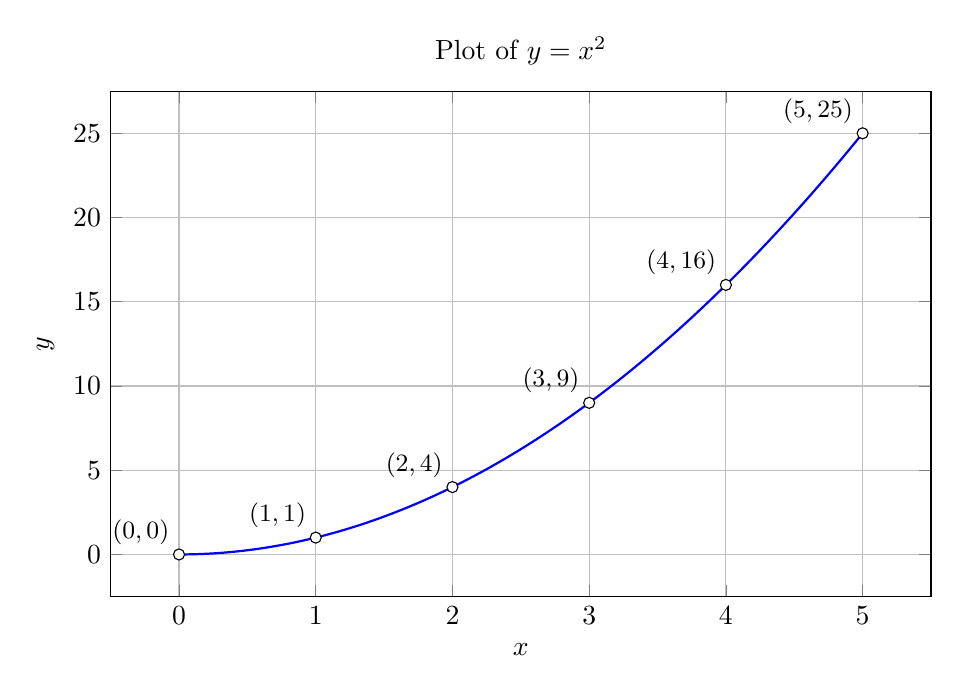
\begin{tikzpicture}
\begin{axis}[
    title={Plot of \( y = x^2 \)},
    xlabel={$x$},
    ylabel={$y$},
    domain=0:5,
    samples=100,
    grid=major,
    width=12cm,
    height=8cm,
    enlargelimits=true,
    xtick={0,1,2,3,4,5},
    ytick={0,5,10,15,20,25},
    every node near coord/.append style={font=\small, anchor=west},
    nodes near coords,
    point meta=explicit symbolic
]

\addplot[
    only marks,
    mark=*,
    mark options={fill=white},
    color=black,
    nodes near coords,
    visualization depends on={point meta'\as\label},
    every node near coord/.append style={anchor=south east}
]
coordinates {
    (0,0) [$(0,0)$]
    (1,1) [$(1,1)$]
    (2,4) [$(2,4)$]
    (3,9) [$(3,9)$]
    (4,16) [$(4,16)$]
    (5,25) [$(5,25)$]
};

\addplot[blue, thick] {x^2};

\end{axis}
\end{tikzpicture}
\end{center}

\end{document}
